\section{High level system overview}
This section addresses high level system design especially.
\begin{itemize}
    \item data structure and data flow
    \item sequential interaction between the system subcomponents
    \item superficial fault tree analysis
    \item software interface definitions
\end{itemize}
The information gathered will be used to derive system requirements \ref{sec:system_requirements}.

\subsection{Data structure and data flow}
We propose the following characteristics for the IMU. Those are inspired for \cite{lm6ds3}. This is a MEMS IMU that is neither a space grade nor UART capable, but provide good characeristic of a basic IMU.

We assume that the IMU will provide the following data:
\begin{itemize}
    \item $a_x$ acceleration on the x-axis
    \item $a_y$ acceleration on the y-axis
    \item $a_z$ acceleration on the z -axis
    \item $\omega_x$ angular rate along its x-axis
    \item $\omega_y$ angular rate along its y-axis
    \item $\omega_z$ angular rate along its z-axis
    \item $T$ temperature of the sensor.
\end{itemize}
From this we derive requirements \linkreq{1}.
We assume that the physical sampling of all those values are made at the exact same time, respectively the difference between the sampling time is negligible.
In other word we can timestamp the measurment time with a single timestamp $t_{mes}$.
% file:///home/mhaselbauer/Downloads/lsm6ds3tr-c.pdf
All values are represented by 16 bits values, sent on the UART protocol in 2 bytes, with the least significant byte first.
The temperature sensor has a sensitivity with 256 LSB $^{\circ}C$.
We assume the IMU would be configure with:
\begin{itemize}
    \item a range of $\pm 16g$ for the accelerometer. The sensitivity is $0.488~mg/LSB$
    \item a range of $\pm 250^{\circ}/s$ for the gyroscope. The sensitivity is $8.75~mdps/LSB$
    \item a output data rate of 208 Hz.
\end{itemize}

We can obtain the physical values from their 16 bits representation from using the following formula.
\begin{equation}
    a = \frac{raw}{2^{15}} \times 16
\end{equation}
\begin{equation}
    \omega = \frac{raw}{2^{15}} \times 250
\end{equation}
\begin{equation}
    T^{\circ_C} = 25+\frac{raw}{256}
\end{equation}
From this we derive \linkreq{2}, \linkreq{3} and \linkreq{4}.




\subsection{Sequential interaction}
The system has following components:
\begin{itemize}
    \item the IMU itself.
    \item the UART peripheral of the compute platform.
    \item the operating system kernel.
    \item the device file that will be created by the kernel to describe the device.
    \item the IMU driver software component.
    \item the IMU message queue.
    \item the odometry application that will consume the IMU data.
\end{itemize}

\begin{figure}[H]
    \centering
    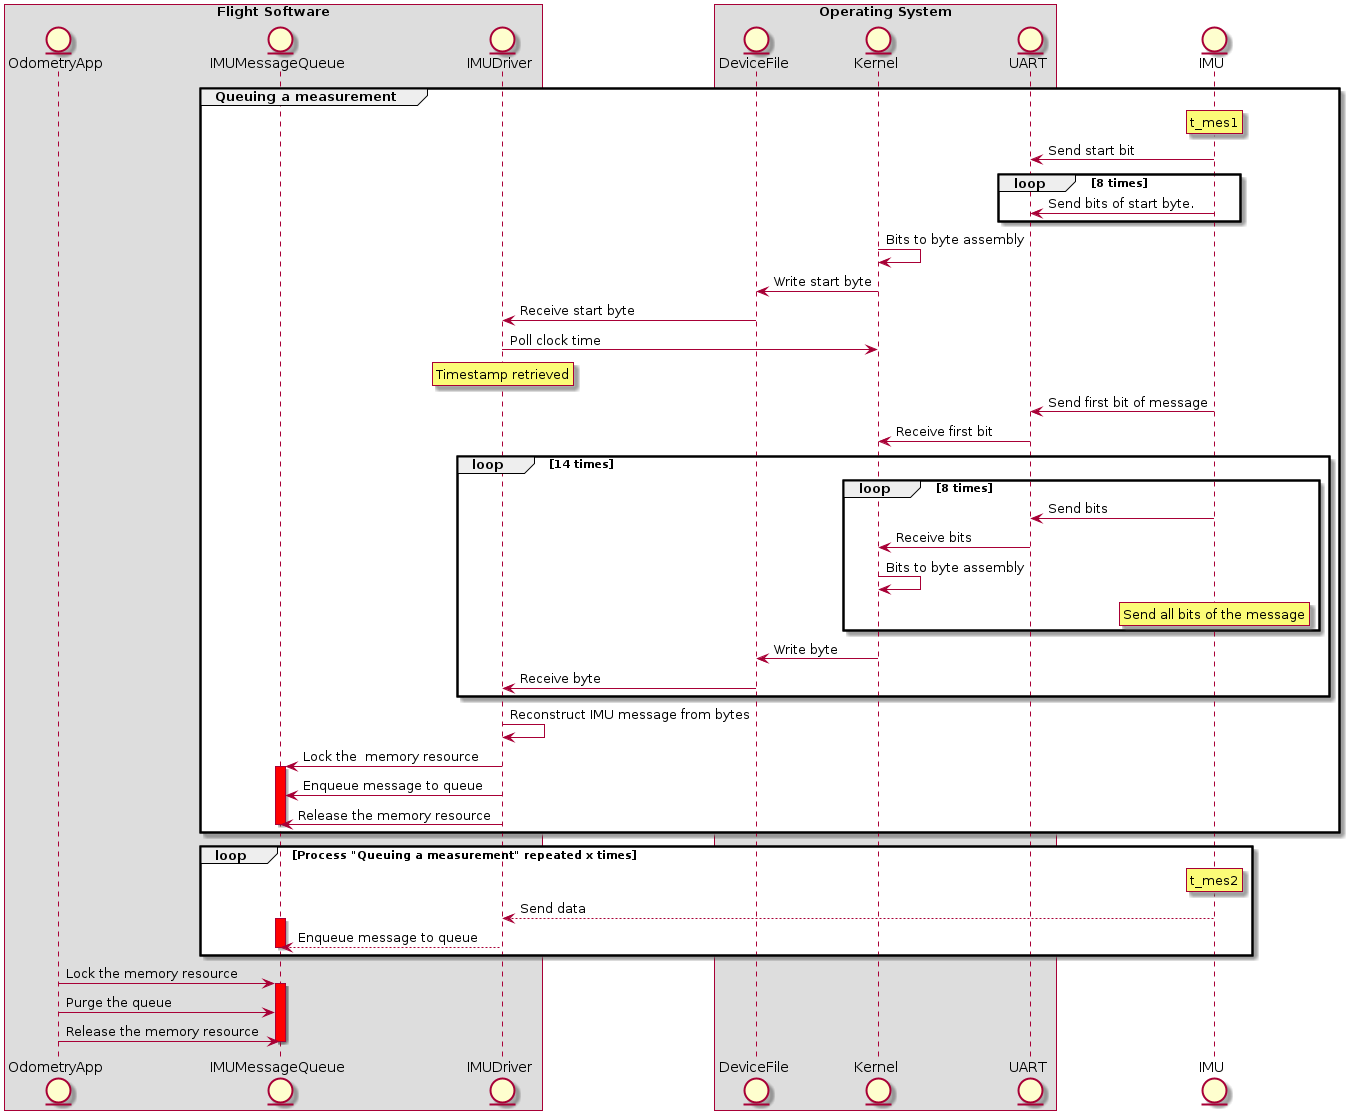
\includegraphics[width=1.0 \textwidth]{diagrams/high_level_sys_overview.png}
    \caption{High level sequence diagram of the nominal operation case}
    \label{fig-high-level-nominal}
\end{figure}

Fig.\ref{fig-high-level-nominal} describe the interaction sequence in the normal operation mode:\\
The IMU makes a new measurment at $t_{mes1}$.
It then sends a start byte to the UART to notify receiver of upcomming data frame.
When the first 8 bits of the start byte have been received, the low level UART driver of the kernel will write the byte to the device file.
The IMU driver will read this and recognize the start of a new data frame (\linkreq{9}).
The IMU driver will then poll the clock time and use it to timestamp the measurement (\linkreq{5}).
The rest of the bytes are collected and then reconstructed into an IMU message.\\
The execution of the IMU driver shall not block the OdometryApp. Thus they must run in separate threads (\linkreq{6}).
To exchange data with the OdometryApp, the IMU driver shall store data in a shared memory queue (\linkreq{7}).\\
This process is repeated several times until the OdometryApp purge all message stored in the queue.\\
The OdometryApp will then process the IMU messages using there value and timestamp.
Therefore the driver must save timestamps together with each coresponding IMU messages (\linkreq{8}).

\subsection{Fault-tree analysis}
Because the IMU Driver is functional safety critical, it is important to derive the relevant technical safety requirements.
This section does not intend to create an exhaustive hazard and risk analysis with all possible failure modes.
This shall be done once the real hardware and usecases are known.
Instead, its intend is to create a superficial fault tree analysis to derive some of the most obvious safety relevant requirements.
We follow a top-down approach postulating a wrong trajectory reconstruction in the OdometryApp as the top event.
We categorize events as green where mitigations measures shall happens outside the IMU driver and red where the IMU driver shall provide the mitigation.

\begin{figure}[H]
    \centering
    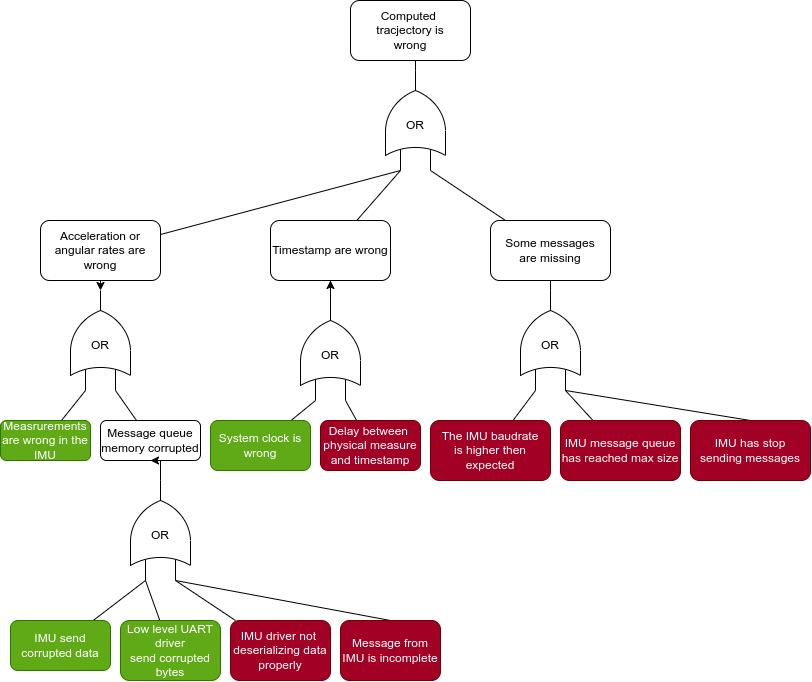
\includegraphics[width=1.0 \textwidth]{diagrams/main_fault_tree.drawio.png}
    \caption{Superficial trajectory reconstruction fault tree.}
    \label{fig-main-fault-tree}
\end{figure}

\begin{center}
\begin{tabular}{|p{5cm}|p{10cm}|}
\hline
\textbf{Failure mode} & \textbf{Mitigation} \\
\hline
IMU driver not deserializing data properly. & shall be addressed by rigorous unit testing of the implementation. \\
\hline
Message from IMU are incomplete. & shall be address by \linkreq{TS1}. \\
\hline
The IMU baudrate is higher than expected & in this simple example, the mitigation consist in notifying the OdometryApp when it collect the IMU messages (\linkreq{TS2},\linkreq{TS3},\linkreq{TS4}). \\
\hline
The IMU message queue has reached max size & the queue shall not grow indefinitely to prevent memory allocation issue(\linkreq(TS8)). The mitigation for the possible drop of message consist in notifying with a counter of dropped message (\linkreq{TS5},\linkreq{TS6}). \\
\hline
The IMU has stop sending messages & the mitigation consist in setting the status to NO\_DATA (\linkreq{TS3},\linkreq{TS7}). \\
\hline
\end{tabular}
\end{center}


\subsection{Software interface definition}
We define the following structure for IMU messages.\\
To fullfill \linkreq{1}, \linkreq{8} and \linkreq{NF1},
\begin{lstlisting}[style=cppstyle]
struct ImuData {
    float a_x{};
    float a_y{};
    float a_z{};
    float omega_x{};
    float omega_y{};
    float omega_z{};
    float temperature{};
    std::chrono::nanoseconds timestamp{};
};
\end{lstlisting}
\textbf{Note:} on x86 the float type is 32 bits long which is more than the strictly necessary 16 bits. We keep float type to be compliant with the C++17 standard library.
There is no requirements on the resolution of the timestamp. This shall be derived from the actual use cases of the OdometryApp.
For the sake of higher accuracy we choose nanoseconds.
Since the measurement would come at 208 Hz only we could potentially microseconds or even miliseconds.\\

To fulfill \linkreq{TS8} and \linkreq{TS5}.
\begin{lstlisting}[style=cppstyle]
struct ImuDataQueue {
  std::uint32_t dropped_message{0};
  SizedCapedQueue<ImuData> data_queue{};
};
\end{lstlisting}

To fulfull \linkreq{TS2}, \linkreq{TS3}, \linkreq{TS7},
\begin{lstlisting}[style=cppstyle]
enum class ImuDriverStatus { OK, BUSY, NO_DATA };
\end{lstlisting}


\subsubsection{Data frames}
Every bytes is transmitted in a UART frame of 10 bits (1 start bit, 8 data bits, 1 stop bit).
\newline
\newline
\begin{bytefield}[bitwidth=4.1em]{10}
    \bitheader[endianness=little]{9,8,1,0}\\
    \bitbox{1}{Start bit}
    \bitbox{8}{Data bits}
    \bitbox{1}{Stop bit}
\end{bytefield}

The IMU transmit 1 start bytes and then 7 values of 2 byte eachs (14 data bytes in total).
The complete message consist if 15 frames: 1 start frame (S) and 14 data frames (D1 to D7).
\newline
\newline
\begin{bytefield}[bitwidth=2.1em]{15}
    \bitheader[endianness=little]{14,1,0}\\
    \bitbox{1}{S}
    \bitbox{14}{D1 to D7}
\end{bytefield}

This amount to 150 bits per message.
With an output data rate of 208 Hz, the required data rate is 31200 bit/s.
We choose a typical baudrate of 38400 bit/s.
This lead to a bit transmission duration of 26 $\mu$s.
The complete message (150 bits) transmission duration is 3906 $\mu$s.
With 208 Hz, the duration between the start of two messages is 4897 $\mu$s.
This leads to an approximative 900 $\mu$s of idle time between two messages.
